\documentclass[12pt]{article}

\usepackage{graphicx}
\graphicspath{ {../Images} }
\usepackage{hyperref}
\usepackage{placeins}
\usepackage{geometry}
\geometry{includeheadfoot,a4paper, textwidth=0.87\paperwidth, textheight=0.9\paperheight, headsep =30pt}
\usepackage[onehalfspacing]{setspace}
\usepackage{fancyhdr}
\pagestyle{fancy}
\renewcommand{\headrulewidth}{1.5pt}
\lhead{
\includegraphics[scale=0.05]{SB.png}}
\rhead{
\includegraphics[scale=0.1]{IDL.png}}
\chead{Docking methods}
\usepackage[super]{natbib}
\usepackage{mol2chemfig}
\usepackage{chemfig}
\usepackage{enumerate}

\begin{document}	
	\title {Docking Methods}
	\date{iGEM Design League 2022}
	\author{Synthetic Biobots\\Gerardo Cendejas Mendoza}
	
	\maketitle

	\begin{center}
		
\includegraphics[scale=0.4]{SB.png}
	\end{center}

	\newpage
	
	\section*{Introduction}
	
	In this document is shown the docking methodology followed by the team  Synthetic Biobots during the iGEM Design League 2022 season. Molecular docking is a process to couple proteins with their ligands; for this project molecular docking was performed in order to support the decision of using the proteins that were selected as part of the biosynthetic pathway of piperamide. The different steps necessary for its production are shown in the Fig. \ref{fig1}; in this figure all the steps required are marked with a number, this number is an identifier for the enzyme required to perform that step.\\
	
	From all the enzymes used in the pathway, only 8 require a docking step for different reasons, these reasons can be that it is an enzyme that has not been isolated and even though a previous annotation step indicates it performs that reaction, molecular docking can provide better support for their selection and activity. Another reason to perform molecular docking is when the protein is known and has been isolated but we are using a molecule that is not the original ligand of the protein, in this case molecular docking can help to elucidate if the protein would be able to perform the reaction with a molecule with similar structure to its' original ligand. The enzymes that are subject of molecular docking and the genes that code for these enzymes and will be studied are: 1 (Pn8.2617), 2 (Pn2.84), 4 (Pn1.1317), 5 (Pn3.4770, Pn7.1626), 6 (Pn16.1237, Pn16.1198), 8 (Pn4.3222), 9 (Pn2.2377) and 10 (\href{https://www.rcsb.org/structure/2CWH}{2cwh}).\\
	
	For each of these genes it was performed a differential exon usage analysis between four different \textit{Piper nigrum} tissues: fruit at 20 days stage, fruit at 40 days stage, leaf and panicle. This analysis can help us to visualize the expression level for each exon of the genes, with this information we can select the exons of the gene to include in the modeling and in the next steps. This analysis was performed using the Bioconductor library ``DEXSeq'', to see the code of this methodology please visit the GitHub repository of the team for iGEM Design League 2022 season, the \href{https://github.com/GerardoCMM/Synthetic-Biobots-IGEM-DL-2022/tree/main/Exon_usage}{Exon\_usage} directory.\cite{bioconductor,dexseq,dexseq_2}\ \ In order to carry out the analysis it was necessary to map the RNAseq reads to the reference genome of \textit{Piper nigrum}, this was done using the STAR ultrafast universal RNA-seq aligner on the Galaxy project platform. \cite{genome,star,galaxy}
	
	
	\FloatBarrier
	\begin{figure}[h]
		\centering
		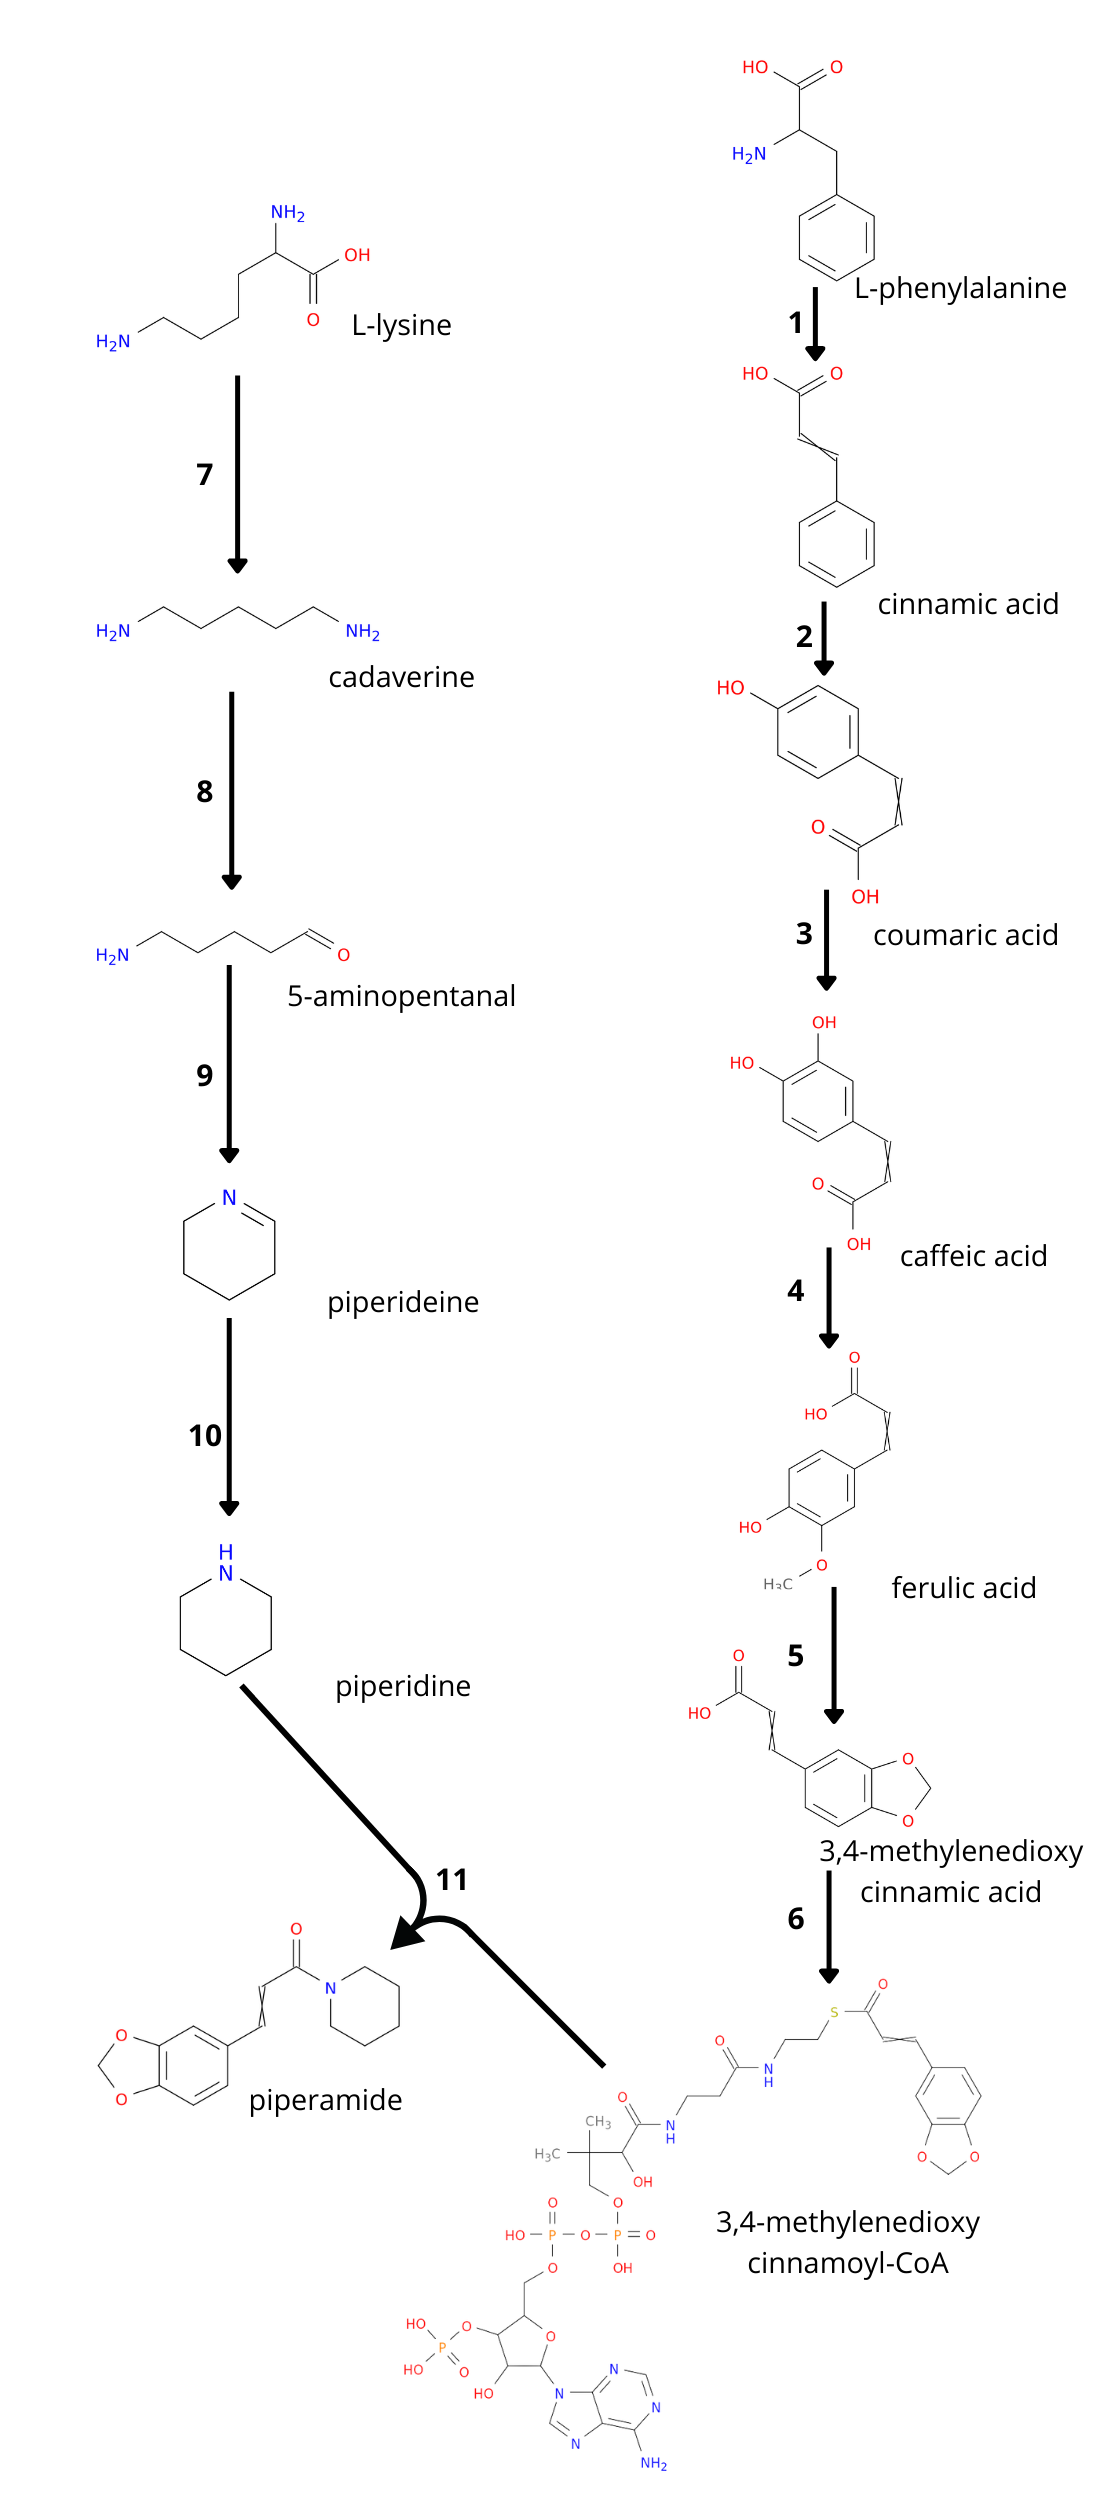
\includegraphics[scale=0.35]{Pathway2.png}
		\caption{Biosynthetic pathway of piperamide.}
		\label{fig1}
	\end{figure}
	\FloatBarrier
	
	\section{Docking}
	
	\subsection{Pn8.2617}
	
	\FloatBarrier
	\begin{figure}[h]
		\centering
		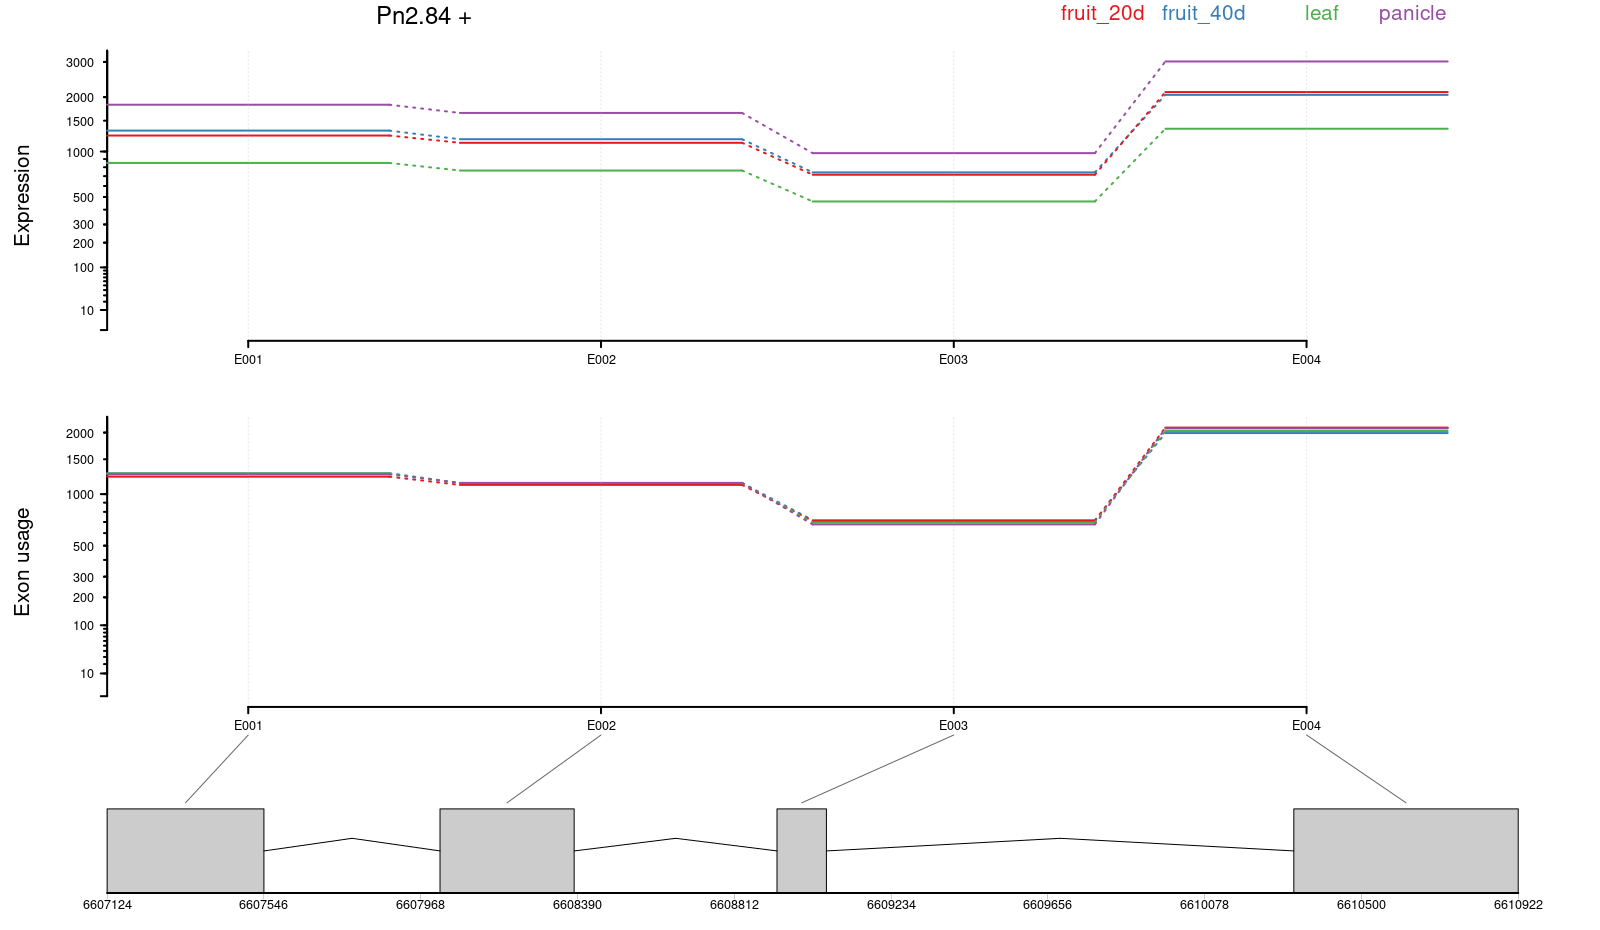
\includegraphics[scale=0.45]{../2/Transcripts/6.png}
		\caption{Algo}
	\end{figure}
	\FloatBarrier
	
	
	
	\begin{center}
		\schemestart
		\chemname{\footnotesize\chemfig{O=[:90](-[:30,,,1]OH)-[:150](-[:90,,,1]NH_2)-[:210]-[:150]-[:90]%
-[:150]-[:210](-[:330,,,,draw=none]\mcfcringle{1.3})-[:270]-[:330](-[:30])}
}{Phenylalanine}\arrow{->[\footnotesize 1]}\chemname{\footnotesize\chemfig{O=[:90](-[:30,,,1]OH)-[:150]-[:210,,,,drh]-[:150]-[:90]-[:150]%
-[:210](-[:330,,,,draw=none]\mcfcringle{1.3})-[:270]-[:330](-[:30])}
}{Cinnamic acid}
		\arrow{0}[,0]\+
		\chemname{\chemfig{NH_3}
}{Ammonia}
		\schemestop
	\end{center}


	\bibliographystyle{apalike}
	\bibliography{references.bib}
	
\end{document}